%%%%%%%%%%%%%%%%%%%%%%%%%%%%%%%%%%%%
% Slide options
%%%%%%%%%%%%%%%%%%%%%%%%%%%%%%%%%%%%

% Option 1: Slides with solutions

\documentclass[slidestop,compress,mathserif]{beamer}
\newcommand{\soln}[1]{\textit{#1}}
\newcommand{\solnGr}[1]{#1}

% Option 2: Handouts without solutions

%\documentclass[11pt,containsverbatim,handout]{beamer}
%\usepackage{pgfpages}
%\pgfpagesuselayout{4 on 1}[letterpaper,landscape,border shrink=5mm]
%\newcommand{\soln}[1]{ }
%\newcommand{\solnGr}{ }


%%%%%%%%%%%%%%%%%%%%%%%%%%%%%%%%%%%%
% Style
%%%%%%%%%%%%%%%%%%%%%%%%%%%%%%%%%%%%

\def\chp4@path{../../Chp 4}
\input{../../lec_style.tex}

%%%%%%%%%%%%%%%%%%%%%%%%%%%%%%%%%%%%
% Preamble
%%%%%%%%%%%%%%%%%%%%%%%%%%%%%%%%%%%%

\title[Lecture 13]{MA213: Lecture 13}
\subtitle{Module 2: Probability, Random Variables, and Distributions}
\author{OpenIntro Statistics, 4th Edition}
\institute{$\:$ \\ {\footnotesize Based on slides developed by Mine \c{C}etinkaya-Rundel of OpenIntro. \\
The slides may be copied, edited, and/or shared via the \webLink{http://creativecommons.org/licenses/by-sa/3.0/us/}{CC BY-SA license.} \\
Some images may be included under fair use guidelines (educational purposes).}}
\date{}

%%%%%%%%%%%%%%%%%%%%%%%%%%%%%%%%%%%%
% Begin document
%%%%%%%%%%%%%%%%%%%%%%%%%%%%%%%%%%%%

\begin{document}


%%%%%%%%%%%%%%%%%%%%%%%%%%%%%%%%%%%%
% Title page
%%%%%%%%%%%%%%%%%%%%%%%%%%%%%%%%%%%%

{
\addtocounter{framenumber}{-1} 
{\removepagenumbers 
\usebackgroundtemplate{\includegraphics[width=\paperwidth]{../../OpenIntro_Grid_4_3-01.jpg}}
\begin{frame}

\hfill \includegraphics[width=20mm]{../../oiLogo_highres}

\titlepage

\end{frame}
}
}


%%%%%%%%%%%%%%%%%%%%%%%%%%%%%%%%%%%%
% Sections
%%%%%%%%%%%%%%%%%%%%%%%%%%%%%%%%%%%%

\subsection{Review}

\begin{frame}
\frametitle{Last time}

\begin{itemize}
    \item Bernoulli random variables
    \item Bernoulli distribution
    \item Geometric distribution arising from Bernoulli
\end{itemize}

Today we will discuss another distribution related to the Bernoulli, but first let's do some counting review.
\end{frame}

\begin{frame}
\frametitle{Factorials and combinations}

\end{frame}

%%%%%%%%%%%%%%%%%%%%%%%%%%%%%%%%%%%%

\section{Edfinity quiz: Counting review}

%%%%%%%%%%%%%%%%%%%%%%%%%%%%%%%%%%%%

\section{Board work: Deriving the Binomial distribution}

%%%%%%%%%%%%%%%%%%%%%%%%%%%%%%%%%%%%

\section{Binomial distribution}

%%%%%%%%%%%%%%%%%%%%%%%%%%%%%%%%%%%%

\subsection{The binomial distribution}

%%%%%%%%%%%%%%%%%%%%%%%%%%%%%%%%%%%%

\begin{frame}

\dq{Suppose we randomly select four individuals to participate in this experiment. What is the probability that exactly 1 of them will refuse to administer the shock?}
\pause
Let's call these people Allen (A), Brittany (B), Caroline (C), and Damian (D). Each one of the four scenarios below will satisfy the condition of ``exactly 1 of them refuses to administer the shock": \\
\vspace{0.25cm}
\pause
\begin{changemargin}{+1.5cm}{+0cm}
{\footnotesize
\begin{enumerate}
\item[Scenario 1:] $\slot{0.35}{\text{(A) \orange{refuse}}} \times \slot{0.65}{\text{(B) shock}} \times \slot{0.65}{\text{(C) shock}} \times \slot{0.65}{\text{(D) shock}} = 0.0961$
\pause
\item[Scenario 2:] $\slot{0.65}{\text{(A) shock}} \times \slot{0.35}{\text{(B) \orange{refuse}}}\times \slot{0.65}{\text{(C) shock}} \times \slot{0.65}{\text{(D) shock}} = 0.0961$
\pause
\item[Scenario 3:] $\slot{0.65}{\text{(A) shock}} \times \slot{0.65}{\text{(B) shock}} \times \slot{0.35}{\text{(C) \orange{refuse}}}\times \slot{0.65}{\text{(D) shock}} = 0.0961$
\pause
\item[Scenario 4:] $\slot{0.65}{\text{(A) shock}} \times \slot{0.65}{\text{(B) shock}} \times \slot{0.65}{\text{(C) shock}} \times \slot{0.35}{\text{(D) \orange{refuse}}} = 0.0961$
\end{enumerate}
}
\end{changemargin}
\pause
The probability of exactly one 1 of 4 people refusing to administer the shock is the sum of all of these probabilities.
\[ 0.0961+ 0.0961 + 0.0961 + 0.0961 = 4 \times 0.0961 = 0.3844 \]

\end{frame}

%%%%%%%%%%%%%%%%%%%%%%%%%%%%%%%%%%%%

\begin{frame}
\frametitle{Binomial distribution}

The question from the prior slide asked for the probability of given number of successes, \mathhl{k}, in a given number of trials, \mathhl{n}, ($k = 1$ success in $n = 4$ trials), and we calculated this probability as
\[ \#~of~scenarios \times P(single~scenario) \]

\pause

\begin{itemize}

\item $\#~of~scenarios$: there is a less tedious way to figure this out, we'll get to that shortly...

\pause

\item $P(single~scenario) = p^k~(1-p)^{(n-k)}$ \\
{\tiny probability of success to the power of number of successes, probability of failure to the power of number of failures}

\end{itemize}

\pause

The \hl{Binomial distribution} describes the probability of having exactly $k$ successes in $n$ independent Bernouilli trials with probability of success $p$.

\end{frame}

%%%%%%%%%%%%%%%%%%%%%%%%%%%%%%%%%%%%

\begin{frame}
\frametitle{Counting the \# of scenarios}

Earlier we wrote out all possible scenarios that fit the condition of exactly one person refusing to administer the shock. If $n$ was larger and/or $k$ was different than 1, for example, $n = 9$ and $k = 2$:

\pause

\begin{center}
\begin{tabular}{c}
\orange{R}\orange{R}SSSSSSS \\ 
\pause
S\orange{R}\orange{R}SSSSSS \\
\pause
SS\orange{R}\orange{R}SSSSS \\
$\cdots$ \\
SS\orange{R}SS\orange{R}SSS \\
$\cdots$ \\
SSSSSSS\orange{R}\orange{R} \\
\end{tabular}
\end{center}

writing out all possible scenarios would be incredibly tedious and prone to errors.

\end{frame}

%%%%%%%%%%%%%%%%%%%%%%%%%%%%%%%%%%%%

\begin{frame}[fragile]
\frametitle{Calculating the \# of scenarios}

\formula{Choose function}
{
The \hl{choose function} is useful for calculating the number of ways to choose $k$ successes in $n$ trials.
\[ {n \choose k} = \frac{n!}{k! (n - k)!} \]
}

\pause

\begin{itemize}

\item $k = 1$, $n = 4$: ${4 \choose 1} = \frac{4!}{1! (4 - 1)!} = \frac{4 \times 3 \times 2 \times 1}{1 \times (3 \times 2 \times 1)} = 4$

\pause

\item $k = 2$, $n = 9$: ${9 \choose 2} = \frac{9!}{2! (9 - 2)!} = \frac{9 \times 8 \times 7!}{2 \times 1 \times 7!} = \frac{72}{2} = 36$

\end{itemize}

\vfill

\Note{You can also use R for these calculations:}
\begin{beamerboxesrounded}[shadow = true, lower = code body]{}
{\small
\begin{verbatim}
> choose(9,2)
[1] 36
\end{verbatim}
}
\end{beamerboxesrounded}

\end{frame}

%%%%%%%%%%%%%%%%%%%%%%%%%%%%%%%%%%%

% \begin{frame}[fragile]
% \frametitle{Properties of the choose function}

% \pq{Which of the following is false?}

% \begin{enumerate}[(a)]
% \item There are $n$ ways of getting 1 success in $n$ trials, ${n \choose 1} = n$.
% \item There is only 1 way of getting $n$ successes in $n$ trials, ${n \choose n} = 1$.
% \item There is only 1 way of getting $n$ failures in $n$ trials, ${n \choose 0} = 1$.
% \solnMult{There are $n-1$ ways of getting $n-1$ successes in $n$ trials, ${n \choose n-1} = n-1$.}
% \end{enumerate}

% \end{frame}

%%%%%%%%%%%%%%%%%%%%%%%%%%%%%%%%%%%

\begin{frame}
\frametitle{Binomial distribution (cont.)}

\formula{Binomial probabilities}
{
If $p$ represents probability of success, $(1-p)$ represents probability of failure, $n$ represents number of independent trials, and $k$ represents number of successes 
\[P(k~successes~in~n~trials) = {n \choose k}~p^k~(1-p)^{(n-k)} \]
} 


\end{frame}

%%%%%%%%%%%%%%%%%%%%%%%%%%%%%%%%%%%

\begin{frame}

\pq{Which of the following is not a condition that needs to be met for the binomial distribution to be applicable?}

\begin{enumerate}[(a)]
\item the trials must be independent
\item the number of trials, $n$, must be fixed
\item each trial outcome must be classified as a \textit{success} or a \textit{failure}
\solnMult{the number of desired successes, $k$, must be greater than the number of trials}
\item the probability of success, $p$, must be the same for each trial
\end{enumerate}

\end{frame}

%%%%%%%%%%%%%%%%%%%%%%%%%%%%%%%%%%%

\begin{frame}
\frametitle{}

\pq{A 2012 Gallup survey suggests that 26.2\% of Americans are obese. Among a random sample of 10 Americans, what is the probability that exactly 8 are obese?}

\begin{enumerate}[(a)]
\item pretty high
\solnMult{pretty low}
\end{enumerate}

\vfill

\ct{Gallup: \webURL{http://www.gallup.com/poll/160061/obesity-rate-stable-2012.aspx}, January 23, 2013.} 

\end{frame}

%%%%%%%%%%%%%%%%%%%%%%%%%%%%%%%%%%%%

\begin{frame}

\pq{A 2012 Gallup survey suggests that 26.2\% of Americans are obese. Among a random sample of 10 Americans, what is the probability that exactly 8 are obese?}

\begin{enumerate}[(a)]
\item $0.262^8 \times 0.738^2$
\item ${8 \choose 10} \times 0.262^8 \times 0.738^2$
\solnMult{${10 \choose 8} \times 0.262^8 \times 0.738^2$} \soln{\orange{\only<2>{$ = 45 \times  0.262^8 \times 0.738^2 = 0.0005$}}}
\item ${10 \choose 8} \times 0.262^2 \times 0.738^8$
\end{enumerate}



\end{frame}

%%%%%%%%%%%%%%%%%%%%%%%%%%%%%%%%%%%

\begin{frame}
\frametitle{The birthday problem}

\dq{What is the probability that 2 randomly chosen people share a birthday?}

\pause

Pretty low, $\frac{1}{365} \approx 0.0027$.

\pause

\dq{What is the probability that at least 2 people out of 366 people share a birthday?}

\pause

Exactly 1! (Excluding the possibility of a leap year birthday.)

\end{frame}

%%%%%%%%%%%%%%%%%%%%%%%%%%%%%%%%%%%

\begin{frame}
\frametitle{The birthday problem (cont.)}

\dq{What is the probability that at least 2 people (1 match) out of 121 people share a birthday?}

\pause

Somewhat complicated to calculate, but we can think of it as the complement of the probability that there are no matches in 121 people.

\vspace{-0.75cm}

\begin{eqnarray*}
P(no~matches) &=& 1 \times \pr{1 - \frac{1}{365}} \times \pr{1 - \frac{2}{365}} \times \cdots \times \pr{1 - \frac{120}{365}} \\
\pause
&=& \frac{365 \times 364 \times \cdots \times 245}{365^{121}} \\
\pause
&=& \frac{365!}{365^{121} \times (365-121)!} \\
\pause
&=& \frac{121! \times {365 \choose 121}}{365^{121}} 
\pause
\approx 0 \\
\pause
P(at~least~1~match) &\approx& 1
\end{eqnarray*}

\end{frame}


%%%%%%%%%%%%%%%%%%%%%%%%%%%%%%%%%%%

\begin{frame}
\frametitle{Expected value}

\dq{A 2012 Gallup survey suggests that 26.2\% of Americans are obese. \\  

Among a random sample of 100 Americans, how many would you expect to be obese?}

\pause

\begin{itemize}

\item Easy enough, $100 \times 0.262 = 26.2$.

\pause

\item Or more formally, $\mu = np = 100 \times 0.262 = 26.2$.

\pause

\item But this doesn't mean in every random sample of 100 people exactly 26.2 will be obese. In fact, that's not even possible. In some samples this value will be less, and in others more. How much would we expect this value to vary?

\end{itemize}

\end{frame}

%%%%%%%%%%%%%%%%%%%%%%%%%%%%%%%%%%%

\begin{frame}
\frametitle{Expected value and its variability}

\formula{Mean and standard deviation of binomial distribution}
{\[ \mu = np \qquad \qquad \sigma = \sqrt{np(1-p)} \] }

\pause

\begin{itemize}

\item Going back to the obesity rate:

\[ \sigma = \sqrt{np(1-p)} = \sqrt{100 \times 0.262 \times 0.738} \approx  4.4\]

\pause

\item We would expect 26.2 out of 100 randomly sampled Americans to be obese, with a standard deviation of 4.4.

\end{itemize}

\Note{Mean and standard deviation of a binomial might not always be whole numbers, and that is alright, these values represent what we would expect to see on average.}

\end{frame}

%%%%%%%%%%%%%%%%%%%%%%%%%%%%%%%%%%%

\begin{frame}
\frametitle{Unusual observations}

Using the notion that \hl{observations that are more than 2 standard deviations away from the mean are considered unusual} and the mean and the standard deviation we just computed, we can calculate a range for the plausible number of obese Americans in random samples of 100.

\[ 26.2 \pm (2 \times 4.4) = (17.4, 35) \]

\end{frame}

%%%%%%%%%%%%%%%%%%%%%%%%%%%%%%%%%%%

\begin{frame}

\pq{An August 2012 Gallup poll suggests that 13\% of Americans think home schooling provides an excellent education for children.  Would a random sample of 1,000 Americans where only 100 share this opinion be considered unusual?}
\begin{multicols}{2}
\begin{enumerate}[(a)]
\item No
\solnMult{Yes}
\end{enumerate}
\end{multicols}

\only<1>{
\begin{center}
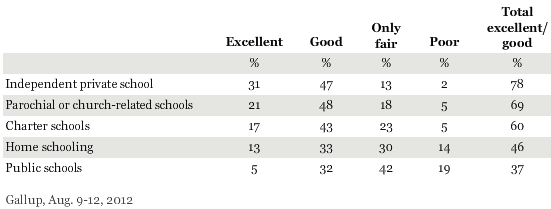
\includegraphics[width=0.8\textwidth]{\chp4@path/4-3_binomial_distribution/figures/homeschool}
\end{center}
}

\vspace{-0.5cm}
\soln{
{\small
\only<2->{
\begin{align*}
\mu &= np = 1,000 \times 0.13 = 130 \\
\sigma &= \sqrt{np(1-p)} = \sqrt{1,000 \times 0.13 \times 0.87} \approx 10.6
\end{align*}
}
\begin{changemargin}{+1cm}{+0cm}
\pause
\begin{enumerate}
\only<3->{\item[Method 1:] Range of usual observations: $130 \pm 2 \times 10.6 = (108.8, 151.2)$ \\
100 is outside this range, so would be considered unusual.}
\only<4->{\item[Method 2:] Z-score of observation: $Z = \frac{x - mean}{SD} = \frac{100 - 130}{10.6} = -2.83$ \\
100 is more than 2 SD below the mean, so would be considered unusual.}
\end{enumerate}
\end{changemargin}
}}

\vfill

\ct{\webURL{http://www.gallup.com/poll/156974/private-schools-top-marks-educating-children.aspx}}

\end{frame}

%%%%%%%%%%%%%%%%%%%%%%%%%%%%%%%%%%%%

\section{R Demonstration: Sampling from the Binomial, Normal Approximation}
% Note: replacing slide below

%%%%%%%%%%%%%%%%%%%%%%%%%%%%%%%%%%%%

% \subsection{Normal approximation to the binomial}

%%%%%%%%%%%%%%%%%%%%%%%%%%%%%%%%%%%%

% \begin{frame}
% \frametitle{}

% \app{Shapes of binomial distributions}
% {
% For this activity you will use a web applet. Go to \webURL{https://gallery.shinyapps.io/dist_calc/} and choose Binomial coin experiment in the drop down menu on the left.
% \begin{itemize}
% \item Set the number of trials to 20 and the probability of success to 0.15. Describe the shape of the distribution of number of successes. 
% \item Keeping $p$ constant at 0.15, determine the minimum sample size required to obtain a unimodal and symmetric distribution of number of successes. Please submit only one response per team.
% \item Further considerations:
% \begin{itemize}
% \item What happens to the shape of the distribution as $n$ stays constant and $p$ changes?
% \item What happens to the shape of the distribution as $p$ stays constant and $n$ changes?
% \end{itemize}
% \end{itemize}
% }

% \end{frame}

%%%%%%%%%%%%%%%%%%%%%%%%%%%%%%%%%%%%

\begin{frame}
\frametitle{Distributions of number of successes}

\dq{Hollow histograms of samples from the binomial model where $p = 0.10$ and $n = 10$, $30$, $100$, and $300$. What happens as $n$ increases?}

\begin{center}
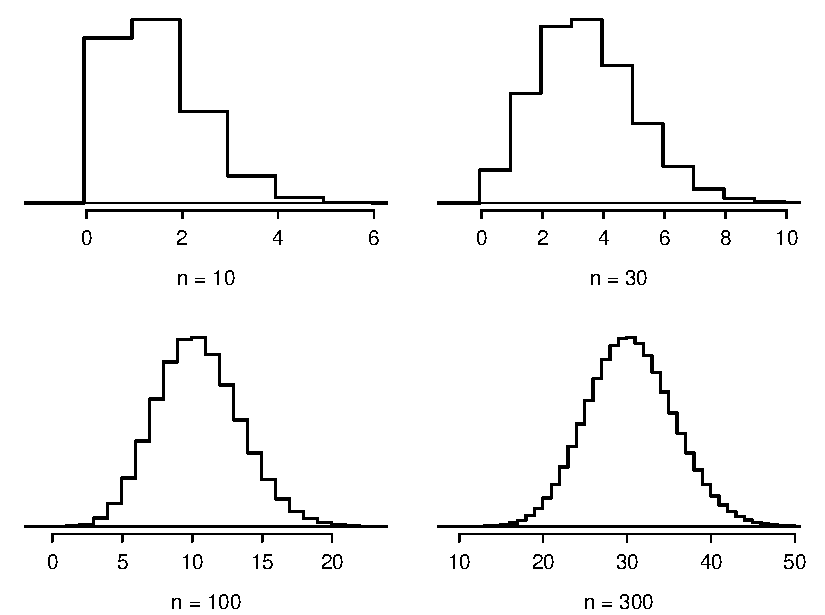
\includegraphics[width=0.60\textwidth]{\chp4@path/4-3_binomial_distribution/figures/fourBinomialModelsShowingApproxToNormal/fourBinomialModelsShowingApproxToNormal}
\end{center}

\end{frame}

%%%%%%%%%%%%%%%%%%%%%%%%%%%%%%%%%%%

\begin{frame}
\frametitle{How large is large enough?}

The sample size is considered large enough if the expected number of successes and failures are both at least 10.
\[ np \ge 10 \qquad \text{ and } \qquad n(1-p) \ge 10 \]

\soln{\only<2->{$10 \times 0.13 = 1.3; 10 \times (1 - 0.13) = 8.7$}}

\end{frame}

%%%%%%%%%%%%%%%%%%%%%%%%%%%%%%%%%%

\begin{frame}
\frametitle{}

\pq{Below are four pairs of Binomial distribution parameters. Which distribution can be approximated by the normal distribution?}

\begin{enumerate}[(a)]
\item $n = 100, p = 0.95$
\solnMult{$n = 25, p = 0.45$} \soln{\only<2>{\orange{$\rightarrow 25 \times 0.45 = 11.25; 25 \times 0.55 = 13.75$}}}
\item $n = 150, p = 0.05$
\item $n = 500, p = 0.015$
\end{enumerate}

\end{frame}


%%%%%%%%%%%%%%%%%%%%%%%%%%%%%%%%%%%%

\section{Edfinity quiz: Modeling with the Binomial distribution}

%%%%%%%%%%%%%%%%%%%%%%%%%%%%%%%%%%%%


% \begin{frame}
% \frametitle{An analysis of Facebook users}

% \dq{A recent study found that ``Facebook users get more than they give". For example:
% \begin{itemize}
% \item 40\% of Facebook users in our sample made a friend request, but 63\% received at least one request
% \item Users in our sample pressed the like button next to friends' content an average of 14 times, but had their content ``liked" an average of 20 times
% \item Users sent 9 personal messages, but received 12
% \item 12\% of users tagged a friend in a photo, but 35\% were themselves tagged in a photo
% \end{itemize}
% Any guesses for how this pattern can be explained?
% }

% \soln{\only<2>{Power users contribute much more content than the typical user.}}

% \ct{\webURL{http://www.pewinternet.org/Reports/2012/Facebook-users/Summary.aspx}}

% \end{frame}

% %%%%%%%%%%%%%%%%%%%%%%%%%%%%%%%%%%%

% \begin{frame}
% \frametitle{}

% \dq{This study also found that approximately 25\% of Facebook users are considered power users. The same study found that the average Facebook user has 245 friends. What is the probability that the average Facebook user with 245 friends has 70 or more friends who would be considered power users? Note any assumptions you must make.}

% We are given that $n = 245, p = 0.25$, and we are asked for the probability $P(K \ge 70)$. To proceed, we need independence, which we'll assume but could check if we had access to more Facebook data.

% \pause

% \begin{align*}
% P(X \ge 70) &= P(K = 70\text{ or }K = 71\text{ or }K = 72\text{ or }\cdots\text{ or } K = 245) \\
% &= P(K = 70) + P(K = 71) + P(K = 72) + \cdots + P(K = 245)
% \end{align*}

% \pause

% This seems like an awful lot of work...

% \end{frame}

%%%%%%%%%%%%%%%%%%%%%%%%%%%%%%%%%%%%

% \begin{frame}
% \frametitle{Normal approximation to the binomial}

% When the sample size is large enough, the binomial distribution with parameters $n$ and $p$ can be approximated by the normal model with parameters $\mu = np$ and $\sigma = \sqrt{np(1-p)}$.

% \begin{itemize}

% \item In the case of the Facebook power users, $n = 245$ and $p = 0.25$.
% \[ \mu = 245 \times 0.25 = 61.25 \qquad \sigma = \sqrt{245 \times 0.25 \times 0.75} = 6.78 \]

% \item $Bin(n = 245, p = 0.25) \approx N(\mu = 61.25, \sigma = 6.78)$.

% \begin{center}
% 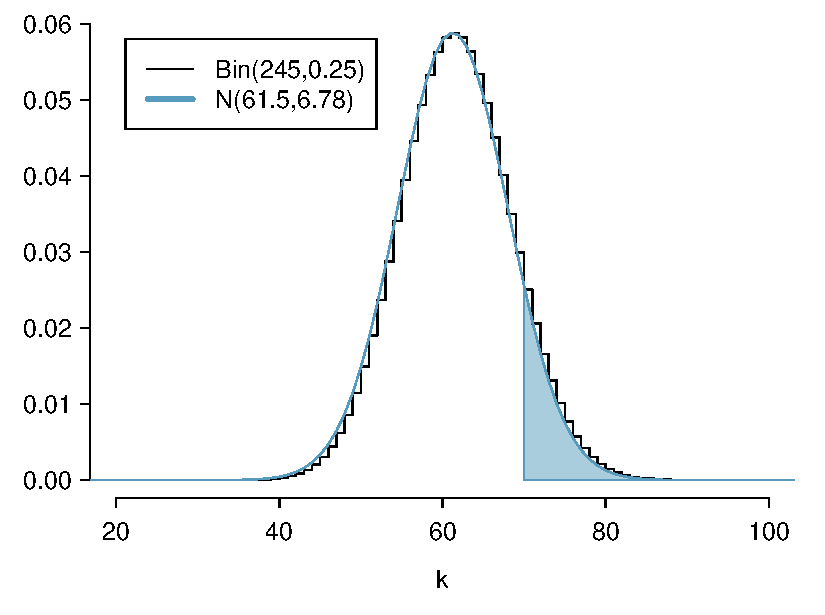
\includegraphics[width=0.5\textwidth]{\chp4@path/4-3_binomial_distribution/figures/fb_power_user/fb_power_user}
% \end{center}

% \end{itemize}

% \end{frame}

%%%%%%%%%%%%%%%%%%%%%%%%%%%%%%%%%%

% \begin{frame}[fragile]
% \frametitle{}

% \dq{What is the probability that the average Facebook user with 245 friends has 70 or more friends who would be considered power users?}

% \pause

% \twocol{0.5}{0.5}{
% \begin{center}
% 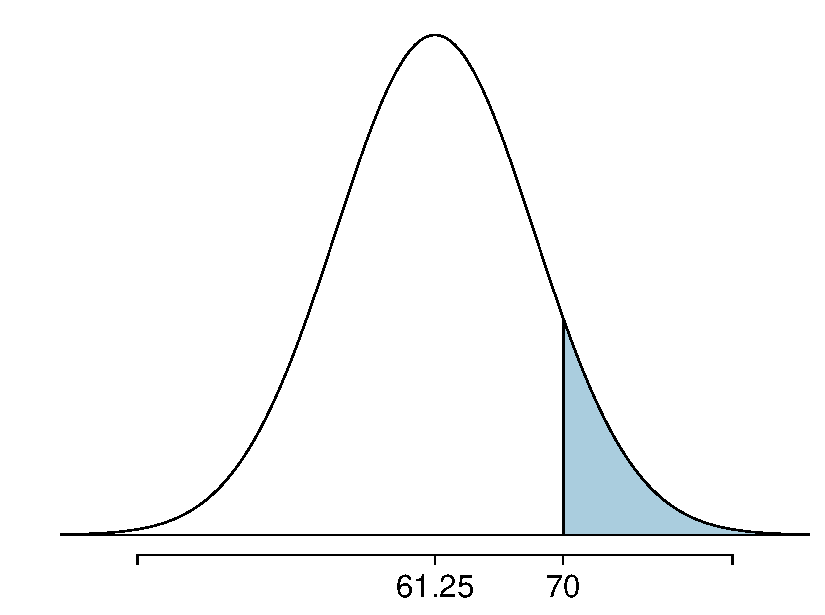
\includegraphics[width=\textwidth]{\chp4@path/4-3_binomial_distribution/figures/fb_power_user/fb_power_user_norm}
% \end{center}
% }
% {
% \[ Z = \frac{obs - mean}{SD} = \frac{70 - 61.25}{6.78} = 1.29 \]
% \[ P(Z > 1.29) = 1 - 0.9015 = 0.0985 \]
% }

% \begin{beamerboxesrounded}[shadow = true, lower = code body]{}
% {\small \begin{verbatim}
% > pnorm(1.29)
% [1] 0.9014747
% \end{verbatim}
% }
% \end{beamerboxesrounded}

% \end{frame}

% %%%%%%%%%%%%%%%%%%%%%%%%%%%%%%%%%

% \subsection{The normal approximation breaks down on small intervals}

% %%%%%%%%%%%%%%%%%%%%%%%%%%%%%%%%%%%%

% \begin{frame}
% \frametitle{The normal approximation breaks down on small intervals}

% \begin{itemize}

% \item The normal approximation to the binomial distribution tends to perform poorly when estimat- ing the probability of a small range of counts, even when the conditions are met.

% \item This approximation for intervals of values is usually improved if cutoff values are extended by 0.5 in both directions.

% \item The tip to add extra area when applying the normal approximation is most often useful when examining a range of observations. While it is possible to also apply this correction when computing a tail area, the benefit of the modification usually disappears since the total interval is typically quite wide.

% \end{itemize}

% \end{frame}

%%%%%%%%%%%%%%%%%%%%%%%%%%%%%%%%%%%

%%%%%%%%%%%%%%%%%%%%%%%%%%%%%%%%%%%%
% End document
%%%%%%%%%%%%%%%%%%%%%%%%%%%%%%%%%%%%

\end{document}